\documentclass[a4paper]{article}
\usepackage{epsfig,epic,eepic,amssymb}
\graphicspath{{FIG/}{PS/}}
\usepackage[francais]{babel}
\usepackage[latin1]{inputenc}
\usepackage{amssymb}
\usepackage{url}
\usepackage{moreverb}
\usepackage{listings}
\addtolength{\parskip}{\baselineskip}
\lstset{language=caml, extendedchars=true}
\newtheorem{theorem}{Theorem}

\usepackage{graphicx}
\usepackage{amsfonts}
\def\C{\mathbb{C}}
\def\N{\mathbb{N}}
\def\Z{\mathbb{Z}}
\def\R{\mathbb{R}}

\begin{document}

\title{\bf TD-TP : QUELQUES VARIANTES SUR LES PLUS COURTS CHEMINS}
\author{Dominique Michelucci, Universit\'e de Dijon}
\date{}

\maketitle

{
\section{TP: PLUS COURTS CHEMINS AVEC DES REPRESENTATIONS MATRICIELLES}
Pour g\'en\'erer le graphe, vous pouvez tirer au hasard des coordonn\'ees de points (
entre 10 et 500, pour simplifier l'affichage).
Vous pouvez refuser de g\'en\'erer des points dans certaines zones, pour simuler des obstacles. 
La longueur des arcs sera
la distance (arrondie sur l'entier  le plus proche si vous le souhaitez) entre les 2 sommets, 
s'ils sont suffisamment proches.

Programmer tous les algorithmes de plus courts chemins vus en cours~:
Ford, Floyd, Dantzig, Dijkstra, pseudo-multiplication de matrice,
en repr\'esentant les graphes par des matrices carr\'ees.
Pour Dijkstra, vous utiliserez un tableau de bool\'eens pour 
savoir si un sommet a \'et\'e "atteint" (la distance \`a la source d'un sommet atteint ne peut plus \^etre modifi\'ee par l'algorithme) ou non. 

Ces algorithmes sont d\'ecrits sur :

\url{http://ufrsciencestech.u-bourgogne.fr/master1/mi1-tc5/COURS_ALGO_HTML/cours_algo017.html}

G\'erez aussi un tableau (ou une matrice) de pr\'ed\'ecesseurs.
Ecrivez une proc\'edure pour reconstituer le plus court chemin jusqu'\`a un sommet donn\`e. 
Vous pouvez stocker le chemin dans un tableau.

Dessinez les ar\^etes du graphe en noir, puis
l'arbre des plus courts chemins en rouge 
(autrement dit les arcs joignant un sommet \`a son pr\'ed\'ecesseur).

\begin{figure}
\begin{center}
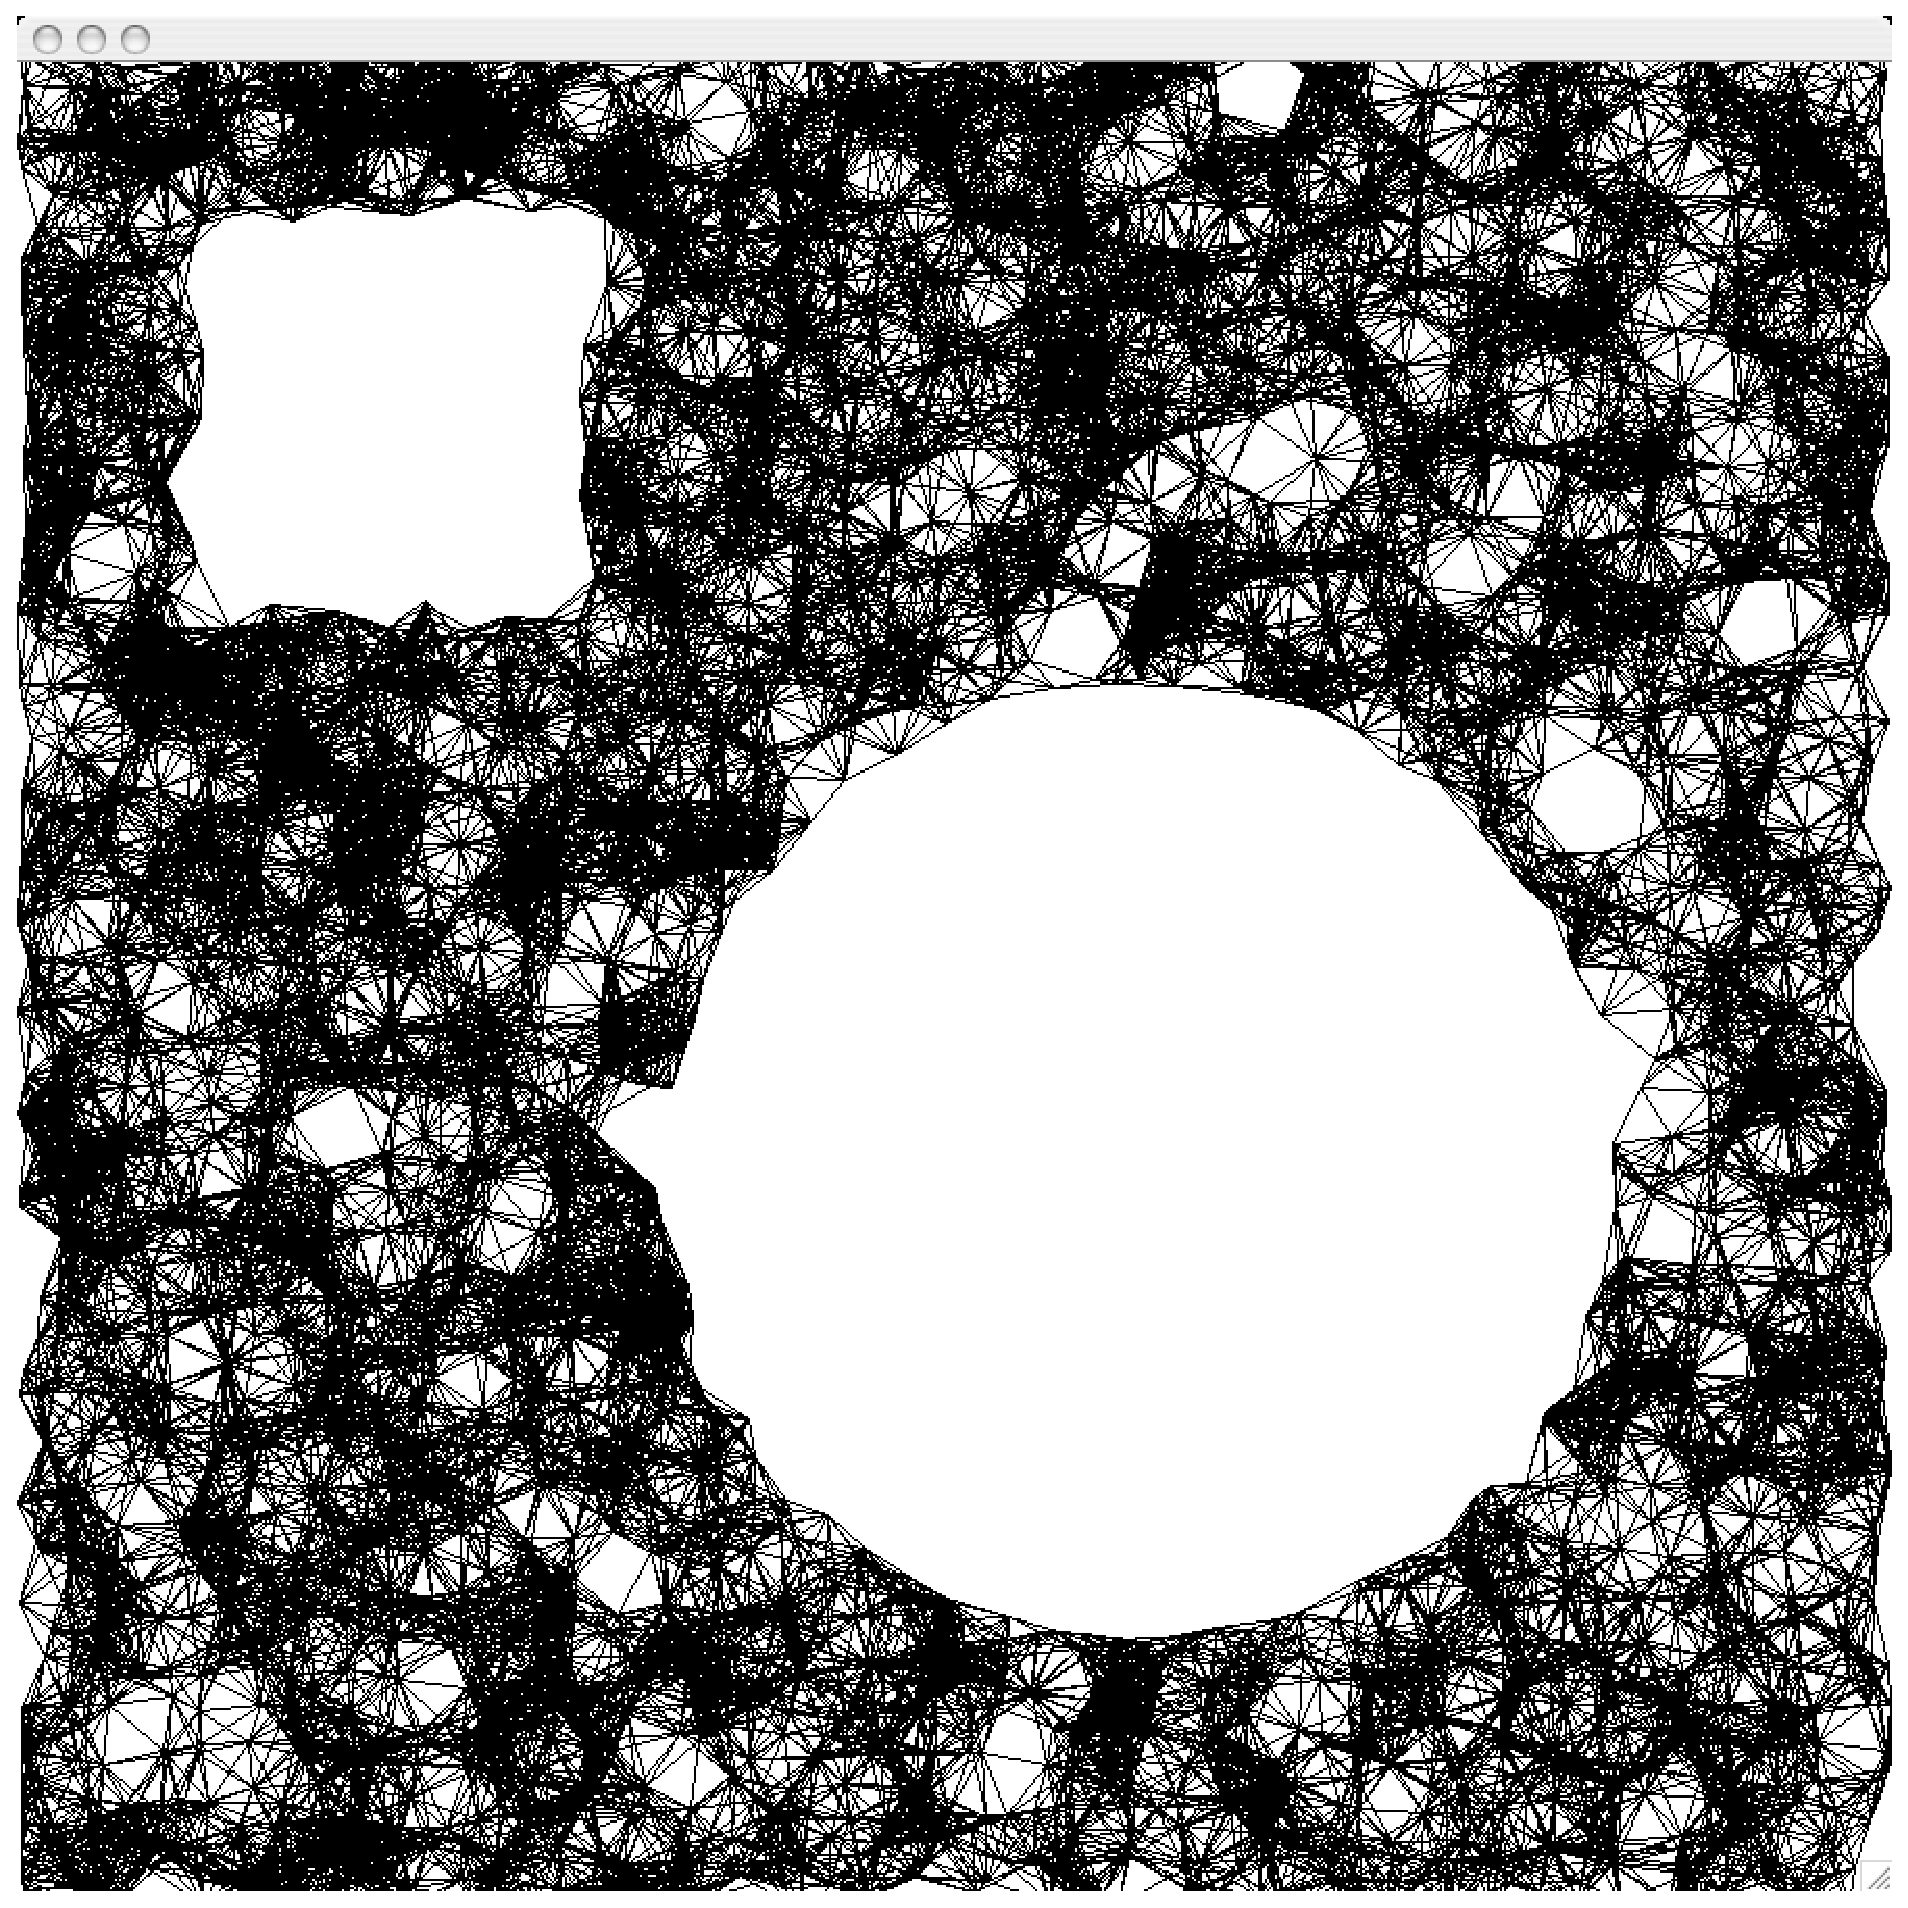
\includegraphics[width=0.45\linewidth]{graphe_PCC.eps}

\includegraphics[width=0.45\linewidth]{arbre_PCC.eps}
\end{center}
\caption{A gauche, le graphe. A droite, l'arbre des plus courts chemins, issus du point en haut \`a gauche (masqu\'e par la banni\`ere de la fen\^etre...). }
\end{figure}

\section{TP: DIJKSTRA AVEC UNE REPRESENTATION PAR LISTE DE VOISINS}
Le m\^eme graphe est ce coup ci repr\'esent\'e par un tableau de liste des arcs~:
$T[s]$ est une liste d'arcs sortant de $s$~; un arc contient les champs~: $t$ un sommet voisin de $s$, et 
$d$ la longueur de l'arc $s\rightarrow t$ (vous pouvez aussi recalculer \`a chaque fois la distance entre les 2 sommets~; ainsi un arc se r\'eduit au num\'ero du sommet $t$ et vous pouvez r\'eutiliser les listes d'entiers...).

Le programme Dijkstra est fourni; mais il utilise une liste et non un tas pour g\'erer les sommets non atteints.
Le programme Heapsort est fourni; il g\`ere un tas, repr\'esent\'e par un tableau. 
Il vous faut modifier le programme
Heapsort pour qu'un sommet (donn\'e par son indice $s$) "connaisse" sa position dans le tas (indication~: utilisez un tableau position[s] qui donne l'indice de la case du tableau/tas qui contient
le sommet num\'ero s; si s n'est plus dans le tas, utiliser l'indice -1. La proc\'edure swap, ou \'echange, doit mettre \`a jour ce tableau position.)
}

\section{ECARTEMENT et METHODE PAC}
Voici une  m\'ethode probabiliste ("probablement approximativement correcte", "Probably Approximately Correct", PAC) pour trouver
une approximation du chemin le plus court entre 2 points $A$ et $B$ quand le graphe est sym\'etrique ($M=M^t$). Echantillonner
l'espace libre, comme dans l'exercice pr\'ec\'edent ; calculer l'arbre des plus courts chemins issus
de $A$, et celui des plus courts chemins 
issus de $B$. L'\'ecartement d'un sommet $S$ est, par d\'efinition,
$AS + SB - AB$ (o\`u $AS, SB, AB$ sont les longueurs des plus courts chemins de $A$ \`a $S$, de $S$ \`a $B$, de $A$ \`a $B$). Si $S$ est sur le plus court chemin de $A$ vers $B$, alors son \'ecartement est nul. Pour pr\'eciser le plus court chemin $AB$, il faut re-\'echantillonner les zones peu \'ecart\'ees du plus court chemin $AB$,   o\`u, par exemple, l'\'ecartement est $10\%$ 
de la longueur du chemin $AB$.
Cette m\'ethode est utilis\'ee en robotique pour la  planification des trajectoires.

{
\section{QUEL EST LE SOMMET SOURCE~?}
Un graphe est donn\'e, par sa matrice des distances (non n\'egatives) entre sommets.
Un sommet source, inconnu, de ce graphe \'emet un signal au temps $0$. Le signal
se propage \`a la vitesse 1 dans le graphe, en utilisant toujours les plus courts chemins.
En quelques sommets, un capteur mesure la date d'arriv\'ee du signal.
Proposez une m\'ethode pour d\'eterminer quel est le sommet source. 
Par exemple, si un capteur est par chance sur le sommet source, il indique la date d'arriv\'ee 0,
et donne donc la source.

M\^eme question, mais la date d'\'emission du signal est inconnue ; seules les dates  
de r\'eception sont connues.

Un algorithme similaire a \'et\'e propos\'e pour d\'eterminer les sources des rumeurs sur internet...

}

\section{CHA\^INES DE MARKOV}
{
\begin{figure}[h]
\begin{center}
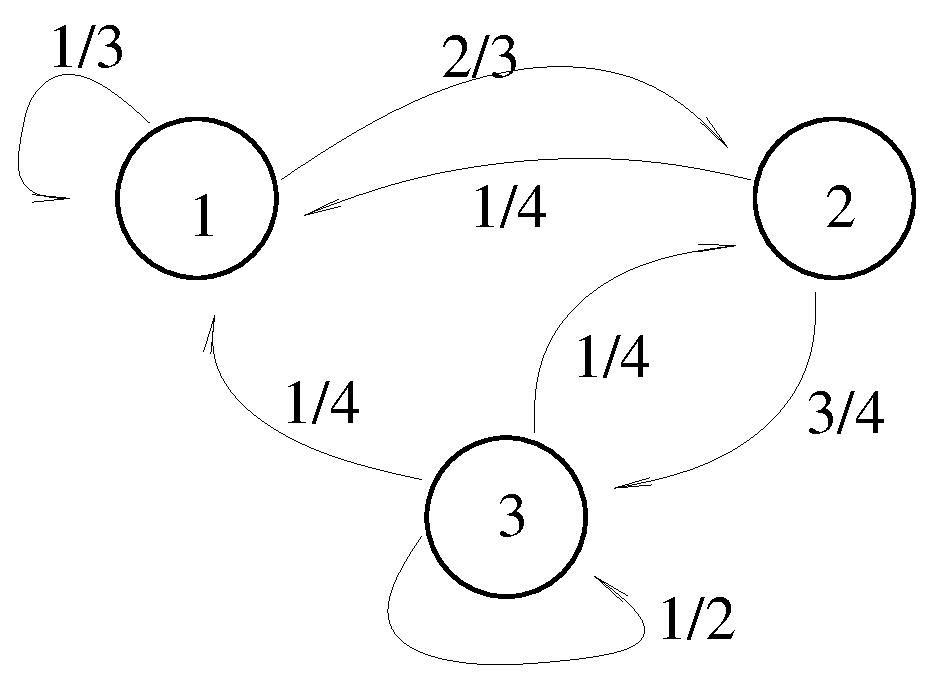
\includegraphics[width=0.4\linewidth]{markov.eps}
\end{center}
\caption{\label{markov} Au premier temps d'internet, il y avait 3 pages, avec les hyperliens ci dessus.
Soit $(p_1, p_2, p_3)$, avec $p_1+p_2+p_3=1$ la distribution de probabilit\'e d'un internaute.
Apr\`es un clic, quelle est la distribution de probabilit\'e~?}
\end{figure}
}
\subsection{Chemin le plus probable}
Les arcs d'un graphe sont \'etiquet\'es par des probabilit\'es ; pour chaque sommet,
la somme des probabilit\'es des
arcs sortants du sommet vaut 1. Ces graphes sont appel\'es cha\^ine de Markov et tr\`es utilis\'es
en math\'ematiques et en informatique (par exemple, pour la reconnaissance automatique de la parole ou des textes, ou comme repr\'esentation des liens entre pages sur Internet). 
Quelle est la probabilit\'e d'un chemin~? 
Comment calculez le chemin les plus probable entre 2 sommets~?

Si vous voulez g\'en\'eraliser la m\'ethode par pseudo produit de matrices, quel
pseudo produit devez vous utiliser pour calculer le chemin le plus probable~?


\subsection{Distribution stationnaire}
Les cha\^ines de Markov ergodiques (irr\'eductibles, non p\'eriodiques) ont une distribution
stationnaire. Calculez celle du graphe de la Fig. \ref{markov}.

Indication:  un clic change la distribution de probabilit\'e $(p_1, p_2, p_3)$ en
$$(p_1', p_2', p_3') = (p_1, p_2, p_3) M, \quad M=\left( \begin{array}{ccc} 1/3 & 2/3 & 0 \\
1/4 & 0 & 3/4 \\
1/4 & 1/4 & 1/2 \\
\end{array}\right)$$
Pour trouver la distribution stationnaire, r\'esolvez $X=XM$ (indication: $(15, 16, 24)=(15, 16, 24)M$).
Informatiquement, on peut calculer $M^{\infty}$ ou bien $M^{2^k}$ avec $k$ "grand"~: $M^{2^k}$
converge assez vite en g\'en\'eral vers une matrice dont toutes les lignes sont \'egales \`a la distribution stationnaire.

Note: au tout d\'ebut, Google utilisait la probabilit\'e stationnaire pour mesurer la pertinence des pages internet... Si $P=PM$, $P_i$ est la probabilit\'e qu'un internaute al\'eatoire se trouve sur la page $i$~: plus $P_i$ est grand (intuitivement~: plus la page est r\'ef\'erenc\'ee, par des pages elles m\^emes bien r\'ef\'erenc\'ee), et plus la page est pertinente. Ce crit\`ere
est manipulable par les plaisantins.


Exemple linguistique~: la probabilit\'e de "mushroom soup" est plus grande que celle de "much rooms hope".
En fran\c{c}ais, consid\'erez~: (sert, sers, cerf, serre) (toi, ta, toit...) (un, hun, hein) (verre, vert, vers...)

Loi de Benford~: en base 10, les nombres commen\c{c}ant par le chiffre 1 sont plus probables~:
empiriquement, ils sont rencontr\'es plus souvent. Voir~:
\url{http://ufrsciencestech.u-bourgogne.fr/master1/mi1-tc5/COURS_ALGO_HTML/cours_algo030.html#toc94}
Par exemple dans la suite 1, 2, 4, 8, 16, 32, 64, 128, 256, 512, 1024, 2048, 4096... il
semble bien que cela soit vrai.
Les cha\^ines de Markov peuvent \^etre utilis\'ees pour calculer les probabilit\'es du premier chiffre dans cette suite.

\section{CHEMIN LE PLUS S\^UR}
Les arcs d'un graphe sont \'etiquet\'es par une probabilit\'e de mourir quand cet
arc est utilis\'e. Quelle est la probabilit\'e de mourir pour un chemin donn\'e~? (Indication~: consid\'erez plut\^ot la probabilit\'e de survie).
Comment calculer le chemin le plus s\^ur entre 2 sommets~? 
Si vous voulez g\'en\'eraliser la m\'ethode par pseudo produit de matrices, quel
pseudo produit devez vous utiliser pour calculer le chemin le plus s\^ur~?


\end{document}

